\section{Contraint Programming}

\subsection{Overview}

Constraint programming is a programming paradigm where problems are modeled as contraints
on variables. That is, a problem is solved by first identifying the variables, the domain
of each variable and the \textit{constraints} of the variables, i.e. the relation between them.
This is different from conventional programming paradigms because you are essentially
describing a solution to the problem, rather than an algorithm on how to achieve the solution.

Contraint programming is used to solve combinatorial problems in a relatively efficient
manner, which makes it an excellent approach to e.g. NP-problems. Constraint programming
is somtimes also called \textit{combinatorial optimization}, and implementations are then
% https://developers.google.com/optimization/
called \textit{combinatorial optimization software suite}. This is perhaps an ever better
name for the paradigm since it describes the usage (and limitations).

% https://en.wikipedia.org/wiki/Constraint_programming#Constraint_programming_libraries_for_imperative_programming_languages
This paradigm is not limited to certain languages but are usually implemented as libraries
that implement a constraint solver. There are also a few languages that support constraint
programming natively, such as Curry.
% http://www-ps.informatik.uni-kiel.de/currywiki/_media/documentation/report.pdf
% http://www-ps.informatik.uni-kiel.de/currywiki/documentation/features
In both cases the user specifies the variables and
the constraints and the constaint solver propagates the given constraints and reduces each
variable's domain until there is only one option left, and the problem is solved.

\subsection{Modeling a Problem}

To illustrate how to model and solve problems with constraint programming consider the
following example.

We are presented with the problem of solving the equation $SEND + MOST = MONEY$, where
each letter is to be subsituted with a digit, $S$ and $M$ cannot be 0, and all digits must
be pairwise distinct. We can easily determine that this is indeed a combinatorial problem
and that, presumably, there exists multiple solutions. The naive method of solving this
problem would be with an exhaustive search. However, this would try a lot of combinations
that can analytically be determined to \textit{not} be part of a solution. To do better we
will employ constraint programming and model the problem in 4 steps:

\begin{enumerate}
	\item Identifying variables and corresponding domains
	\item Determining constraints
	\item Choosing a search heuristic
	\item Optimizing
\end{enumerate}

\subsubsection{Identifying Variables and Corresponding Domains}

The first step of modeling is to determine the variables of the problem, and what their
possible values are. The set of possible values is refered to as the variable's \textit{
domain}. Choosing the variables of a problem is not always easy and the implications
of the choice may not be apparent until later steps. E.g. for certain problems the intuitive
variable selection might make searching too inefficient to ever terminate. In our case
choosing variables is very straightforward. We have one variable for each letter. Since
each letter is the be replaced with a digit the domain of each variable is 0 through 9.

\vspace{0.5cm}
\noindent
$S \in \{0, 1, 2, 3, 4, 5, 6, 7, 8, 9\}$ \\
$E \in \{0, 1, 2, 3, 4, 5, 6, 7, 8, 9\}$ \\
$N \in \{0, 1, 2, 3, 4, 5, 6, 7, 8, 9\}$ \\
$D \in \{0, 1, 2, 3, 4, 5, 6, 7, 8, 9\}$ \\
$M \in \{0, 1, 2, 3, 4, 5, 6, 7, 8, 9\}$ \\
$O \in \{0, 1, 2, 3, 4, 5, 6, 7, 8, 9\}$ \\
$T \in \{0, 1, 2, 3, 4, 5, 6, 7, 8, 9\}$ \\
$Y \in \{0, 1, 2, 3, 4, 5, 6, 7, 8, 9\}$

Henceforth two integers seperated by two dots will indicate a range of all integers between
and including the two specified.

\subsubsection{Determining Constraints}

The constraints of our model is used to describe the relationship between variables in a
solution. For example how does $S$ and $E$ interact when part of a solution? Given the
problem describtion one constraint is that each digit is only used once, i.e. our variables
are pairwise distinct. If $S$ is assigned 1, no other letter can be assigned 1. In addition,
both $S$ and $M$ are nonzero, so we post one constraint for each that excludes 0 from their
domain.

To enforce the equation in the problem description we post the constraint: \\

\begin{tabular}{cccccc}
	& & $1000 * S$ & $100 * E$ & $10 * N$ & $D$ \\
	+ &	& $1000 * M$ & $100 * O$ & $10 * S$ & $T$ \\
	\hline
	& $10000 * M$ & $1000 * O$ & $100 * N$ & $10 * E$ & $Y$
\end{tabular}

If all of these constraints are true for a certain mapping of letters to digits, that
mapping is considered a solution to the problem.

\subsubsection{Propagating}

To find a solution we start by \textit{propagating} these constraint. Propagating a constraint
means that for every constraint we check which values in a variable's domain are incompatible
with the constraint. I.e. we exclude values that can never be part of a solution. In this
case, we have one constraint for $S$ and one constraint for $M$ that say that they must
be nonzero. We can thus remove the 0 from their domains. We systematically work through
all constraints and keep pruning values from domains.

% TODO The variables and their domains after propagation for the example
If we propagate the given constraints on the initial domains of our variables we are left
with the following state:

\vspace{0.5cm}
\noindent
$S \in \{9\}$ \\
$E \in \{2..7\}$ \\
$N \in \{3..8\}$ \\
$D \in \{2..8\}$ \\
$M \in \{1\}$ \\
$O \in \{0\}$ \\
$T \in \{2..8\}$ \\
$Y \in \{2..8\}$

Notably, we have already determined that $S$ has to be 9, which excludes it from all other
domains. In a similar manner we have assigned $M=1$ and $O=0$ and removed 1 and 0 from all
other domains, this in turn has led to the exclusion of 2 from the domain of $N$. In other
words, the equation will look something like $9END + 109T = 10NEY$

When no more domains can be pruned we have one of three situations. One or more domain(s)
could be empty, proving that no solution exists. All domains could be of size 1, indicating
that there exists only one possible value for every variable, and thus we have found a
solution. And last but not least, one or more variables have multiple values in their
domain. If we reach any of the former situations, either a solution is found or we have proven
that a solution does not exist. In the latter situation we have multiple possbile values,
and we must explore these combinations. We do that by \textit{branching}.

\subsubsection{Searching}

To explore the different combinations of variable to value mappings we construct a \textit{
search tree}. Each node of the search tree constists of every variable and their respective
domain after propagation. The root node would then be the all variables and their domains
after initial propagation (as in the previous section). From each node we create two or
more branches, where each branch represents a subset of a domain for a particular variable.
For example, we could create one branch were $E \in \{2..4\}$ and one branch where $E \in 
\{5..7\}$. It is important that the branches completely covers the original
domain, so that all possible values are explored.

We will then follow one of the branches, propagate constraints given the reduced domain
of the branching variable and once again reach one of the three previously mentioned
situations, only in this case if we have reached the first situation (failure) we can go
back and go down the other branch. This process is applied recuresively until a solution
is found or all combinations have been exhausted.

\subsubsection{Choosing a branching heuristic}

Determining on which variable to branch, how many branches to create and which values to
include or exclude for every branch is very much dependent on the problem being modeled.
In this case something simple is sufficient and we can say that when a dead-end is reached
we pick the variable with the smallest domain and create one branch where that variable
is mapped to the smallest value in that domain, and one branch where the smallest value
is excluded from the domain.

\begin{figure}[h]
	\centering
	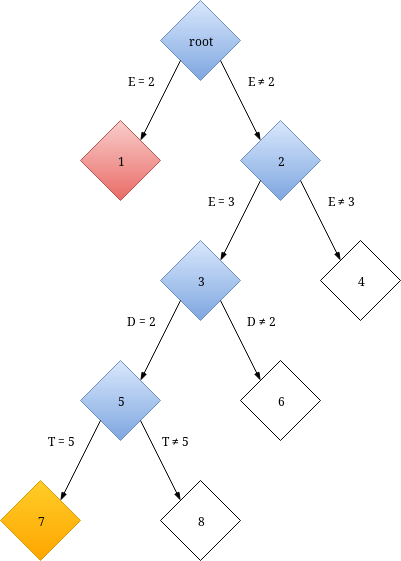
\includegraphics[width=8cm]{background/figures/constraint_first_solution}
	\caption{Search tree of first solution to SEND+MOST=MONEY problem.
	White nodes are unvisited, blue nodes are propagated, red nodes are failed and orange nodes are solutions.}
	\label{fig:first_solution}
\end{figure}

\begin{table}
	\centering
	\begin{tabular}{c|c|c|c|c|c|c|c|c}
		Node & S & E & N & D & M & O & T & Y \\
		\hline
		root & 9 & {2..7} & {3..8} & {2..8} & 1 & 0 & {2..8} & {2..8} \\
		2 & 9 & {3..7} & {4..8} & {2..8} & 1 & 0 & {2..8} & {2..8} \\
		3 & 9 & 3 & 4 & {2, 5, 6} & 1 & 0 & {2, 5, 6} & {5..8} \\
		5 & 9 & 3 & 4 & 2 & 1 & 0 & {5, 6} & {7, 8} \\
		7 & 9 & 3 & 4 & 2 & 1 & 0 & 5 & 7 \\
	\end{tabular}
	\caption{Each variable's domain in the nodes (after propagation) explored to reach the first solution}
	\label{tab:first_solution_states}
\end{table}

Figure \ref{fig:first_solution} shows all branching made to reach the first solution given
our branching heuristic. Table \ref{tab:first_solution_states} show the domains of each
variable at a given node (after propagation). Node 7 represents a solution to the problem,
namely $9342+1095=10437$.

\subsubsection{Optimizing}

As previously mentioned constraint programming is sometimes called combinatorial optimization.
Optimizing the solution is done during the search. When we find a solution by searching,
instead of terminating the program and returning the found solution we apply an additional
constraint that says that from now on, a combination will only be considered a solution
if it is \textit{better} than the current solution. If we find another solution, we can
set the bar at that solution instead. This process is called \textit{branch and bound}.

For a combinatioral problem we expect mutliple solutions, and by always requiring the
next solution to be better than the last we will eventually, given enough time, reach
the \textit{optimal} solution. That is if we apply a branch and bound strategy and allow
it to run until termination, we have both found the optimal solution and proved that it is
the optimal solution. For large problems however, this might take an unreasonable amount
of time and it is better to terminate early.

To first step of finding the optimal solution is indentify what constintutes as \textit{
	better}. In our case we want as much money as possible. One solution is better than
another one if the mapping of $MONEY$ yields a larger integer. Table \ref{tab:two_solutions}
shows two distinct solutions, one better than the other.
% Provide example with two solutions

\begin{table}
	\centering
	\begin{tabular}{c|c|c|c|c|c|c|c|c}
		S & E & N & D & M & O & T & Y & MONEY \\
		\hline
		9 & 3 & 4 & 2 & 1 & 0 & 5 & 7 & 10437 \\
		9 & 3 & 4 & 2 & 1 & 0 & 6 & 8 & 10438 \\
	\end{tabular}
	\caption{Two solution to the problem, one better than the other.}
	\label{tab:two_solutions}
\end{table}

For every solution we find, we require subsequent solution to map $MONEY$ to a larger
integer. The optimal solution is the largest integer for $MONEY$ we can find while still
conforming to all constraints. If we keep searching and keep requiring that the next solution
is better than the last we will eventually conclude that the optimal solution is the one
presented in table \ref{tab:optimal_solution}.

\begin{table}
	\centering
	\begin{tabular}{c|c|c|c|c|c|c|c|c}
		S & E & N & D & M & O & T & Y & MONEY \\
		\hline
		9 & 7 & 8 & 2 & 1 & 0 & 4 & 6 & 10876 \\
	\end{tabular}
	\caption{The optimal solution.}
	\label{tab:optimal_solution}
\end{table}

% Source code in appendix TODO: figure out which appendix
The source code, written with Gecode, for the problem can be found in appendix X

\subsection{Summary}
The most important part of constraint programming is that you are describing how a
solution to a problem looks, not how to calculate that solution. This in turn makes it
good for combinatorial problems, where you can quickly exclude certain combinations thanks
to early detection of illegal values. By then creating a \textit{search tree}, where each
node represents a particular state of variables and their respective domains and each
branch represents limiting a variable's domain to a subset of the previous state. When
searching for solutions one can require that the next candidate is only considered a solution
if it is in some way \textit{better} than the previous solution, thus eventually yielding
the optimal solution.
